\documentclass[xcolor=pdftex,dvipsnames,table,mathserif]{beamer}
\usepackage{subfigure}
\usepackage{amsbsy}
\usepackage{tikz}
\usetikzlibrary{arrows}
\usepackage{amsmath,graphicx,dsfont,color}
\usepackage{amsfonts}
\usepackage{amssymb}
\usepackage{array}

\bibliographystyle{apalike}

\setbeamertemplate{bibliography item}{\insertbiblabel}
\setbeamertemplate{bibliography entry title}{}
\setbeamertemplate{bibliography entry location}{}
\setbeamertemplate{bibliography entry note}{}

\DeclareMathOperator*{\argmin}{arg\,min}
\DeclareMathOperator*{\argmax}{arg\,max}
%Definitiona

\newcommand{\x}{\mathbf{x}}
\newcommand{\X}{\mathbf{X}}
\newcommand{\W}{\mathbf{W}} %Weight
\newcommand{\bais}{\mathbf{b}}%Bais
\newcommand{\act}{\texttt{g}}%Activation
\newcommand{\loss}{L}
\newcommand{\pdata}{\hat{p}_{\texttt{data}}}
\newcommand{\nsize}{n}
\newcommand{\param}{\boldsymbol{\theta}}
\newcommand{\featmap}{\boldsymbol{\phi}}
\newcommand{\EV}{\mathbb{E}}







\usepackage{physics}

\graphicspath{{../graphics/}}

\AtBeginSection[]{
  \begin{frame}{Contents}
    \tableofcontents[currentsection, hideothersubsections]
  \end{frame}
}

\AtBeginSubsection[]{
  \begin{frame}{Contents}
    \tableofcontents[currentsection, subsectionstyle=show/shaded/hide]
  \end{frame}
}

\setbeamertemplate{footline}[frame number]{}
\setbeamertemplate{navigation symbols}{}
\setbeamertemplate{section in toc}[square]
\setbeamertemplate{items}[square]

%% For image credits on image bottom right
\usepackage[absolute,overlay]{textpos}
\setbeamercolor{framesource}{fg=gray}
\setbeamerfont{framesource}{size=\tiny}
\newcommand{\source}[1]{\begin{textblock*}{4cm}(8.7cm,8.6cm)
    \begin{beamercolorbox}[ht=0.5cm,right]{framesource}
      \usebeamerfont{framesource}\usebeamercolor[fg]{framesource} Credits: {#1}
    \end{beamercolorbox}
\end{textblock*}}

\title{Deep learning for image analysis quick introduction}
\author{E. Decencière}
\date{MINES ParisTech\\
  PSL Research University\\
  Center for Mathematical Morphology
}
\titlegraphic{
\includegraphics[height=1.7cm]{../graphics/logoemp}}

\useinnertheme{rounded}
\usecolortheme{rose}

%%%%%%%%%%%%%%%%%%%%%%%%%%%%%%%%%%%%%%%%%%%%%%%%%%%%%%%
%%%%%%%%%%%%%%%%%%%%%%%%%%%%%%%%%%%%%%%%%%%%%%%%%%%%%%%

\begin{document}

\frame{\titlepage}

\frame{
  \frametitle{Contents}
  \tableofcontents[hidesubsections]
}

%%%%%%%%%%%%%%%%%%%%%%%%%%%%%%%%%%%%%%%%%%%%%%%%%%
%%%%%%%%%%%%%%%%%%%%%%%%%%%%%%%%%%%%%%%%%%%%%%%%%%
\section{Introduction}

%%%%%%%%%%%%%%%%%%%%%%%%%%%%%%%%%%%%
\begin{frame}{A revolution in image analysis}

\begin{figure}[ht]
  \centering
  \includegraphics[height=0.5\textheight]{lemonde-juillet2015}
  \caption{Le Monde, juillet 2015}
\end{figure}


\end{frame}

%%%%%%%%%%%%%%%%%%%%%%%%%%%%%%%%%%%%
\begin{frame}{A revolution in image analysis}

\begin{figure}[ht]
  \centering
  \includegraphics[height=0.5\textheight]{nature_go}
  \caption{Nature, 2016}
\end{figure}


\end{frame}


%%%%%%%%%%%%%%%%%%%%%%%%%%%%%%%%%%%%
\begin{frame}{A revolution in image analysis}

\begin{figure}[ht]
  \centering
  \includegraphics[width=0.7\textwidth]{lemonde27mars2019}
  \caption{Le Monde, mars 2019}
\end{figure}


\end{frame}


%%%%%%%%%%%%%%%%%%%%%%%%%%%%%%%%%%%%%%%%%%%%%%%%%%
\section{Differentiable programming}


%%%%%%%%%%%%%%%%%%%%%%%%%%%%%%%%%%%%
\begin{frame}{Differentiable programming}

\begin{block}{Definition}
  Differentiable programming is an algorithmic framework where differentiable operators are combined together to build complex systems. The parameters of the system can then be optimized via gradient descent thanks to \alert{back-propagation}.
\end{block}

\begin{itemize}
\item In our case, computational graphs will be used to compute a \alert{loss} function $\loss$, which depends on the input of the system $\X$ and its parameters $\param = \{\param_1, \ldots, \param_q\}$.
\item Example:
  \[
  \loss(\X, \param) = (f_{\param_1} \circ g_{\param_2} + h_{\param_3}) (\X)
  \]

\end{itemize}

\end{frame}
%%%%%%%%%%%%%%%%%%%%%%%%%%%%%%%%%%%%
\begin{frame}{Gradient descent in the scalar case}

\begin{columns}
  \begin{column}{.5\textwidth}
    \includegraphics[width=\textwidth]{gradient_descent}
  \end{column}

  \begin{column}{.5\textwidth}
    \[
    \param_{t+1} = \param_t - \lr\nabla \loss(\param_t)
    \]
  \end{column}
\end{columns}

\end{frame}



%%%%%%%%%%%%%%%%%%%%%%%%%%%%%%%%%%%%
\begin{frame}{How to minimize a function?}

  \begin{columns}
    \begin{column}{.6\textwidth}
      \begin{figure}
        \includegraphics[height=5cm]{3d-gradient-cos.png}
        \source{By MartinThoma, CC0, https://commons.wikimedia.org/}
      \end{figure}
    \end{column}


    \begin{column}{.4\textwidth}
      \begin{block}{Definition: gradient}
        Let $\loss $ be a derivable function from $\R^n$ into $\R$. Its gradient $\nabla\loss$ is:
        \[
        \nabla \loss (\param) =
        \begin{pmatrix}
          \frac{\partial \loss}{\partial \param_1}(\param)\\
          \vdots \\
          \frac{\partial \loss}{\partial \param_n}(\param)
        \end{pmatrix}
        \]

      \end{block}
    \end{column}
  \end{columns}


\end{frame}

%%%%%%%%%%%%%%%%%%%%%%%%%%%%%%%%%%%%
\begin{frame}{Computational graph}

\begin{block}{Definition}
  A computational graph is a direct acyclic graph such that:
  \begin{itemize}
  \item A node is a mathematical operator
  \item To each edge is associated a value
  \item Each node can compute the values of its output edges from the values of its input edges
    \begin{itemize}
    \item Nodes without input edges are \emph{input nodes}. They represent the input values of the graph.
    \item Similarly, output values can be held in the \emph{output nodes}.
    \end{itemize}
  \end{itemize}
\end{block}

Computing a \emph{forward pass} through the graph means choosing its input values, and then progressively computing the values of all edges.


\end{frame}


%%%%%%%%%%%%%%%%%%%%%%%%%%%%%%%%%%%%
\begin{frame}{Computational graph example}
  Computational graph of:
  \[
  \sigma(w_1x + w_2y + b)
  \]
  where $\sigma$ is the sigmoid function: $\sigma(x) = \frac{1}{1 + e^{-x}}$

\vspace{3em}
\pause

  \centering
  \includegraphics[width=0.7\textwidth]{comp_graph2}\\
  \pause
  The graph can be represented at different levels of detail:
  \includegraphics[width=0.7\textwidth]{comp_graph}

\end{frame}

%%%%%%%%%%%%%%%%%%%%%%%%%%%%%%%%%%%%
\begin{frame}{Gradient descent applied to computational graphs}

  In the case of computational graphs, the loss $\loss$ depends on each parameter $\param_i$ via the composition of several simple functions. In order to compute the gradient $\nabla_{\param}\loss$ we will make extensive use of the chain rule theorem.

  \begin{block}{Chain rule theorem}
    Let $f_1$ and $f_2$ be two derivable real functions ($\R \rightarrow \R$). Then for all $x$ in $\R$:   :
    \[
     (f_2 \circ f_1)'(x) = f_2'(f_1(x)).f_1'(x)
    \]
  \end{block}


\begin{block}{Leibniz notation}
  Let us introduce variables $x$, $y$ and $z$:
  \[x \xrightarrow{f_1} y \xrightarrow{f_2} z\]

  Then:
  \[\dv{z}{x} = \dv{z}{y} \cdot \dv{y}{x} \]

\end{block}

\end{frame}


%%%%%%%%%%%%%%%%%%%%%%%%%%%%%%%%%%%%
\begin{frame}{The backpropagation algorithm}

  \begin{itemize}
  \item The backpropagation algorithm is used in a neural network to efficiently compute the partial derivatives of the loss with respect to each parameter of the network.
  \item One can trace the origins of the method to the sixties
  \item It was first applied to NN in the eighties \cite{werbos_applications_1982, lecun_procedure_1985}
  \end{itemize}


\end{frame}


%%%%%%%%%%%%%%%%%%%%%%%%%%%%%%%%%%%%
\begin{frame}{The backpropagation algorithm: intuition}

  \begin{itemize}
  \item Given a computational graph, the main idea is to compute the local partial derivatives during a forward pass
    \item Then, during a backward pass, the partial derivatives of the loss with respect to each parameter is computed
  \end{itemize}


\end{frame}





%%%%%%%%%%%%%%%%%%%%%%%%%%%%%%%%%%%%
\begin{frame}<handout>{Simple backpropagation example}

\includegraphics[width=\textwidth]{bp_simple.png}

\end{frame}

%%%%%%%%%%%%%%%%%%%%%%%%%%%%%%%%%%%%
\begin{frame}<beamer>{Simple backpropagation example}

\only<1>{\includegraphics[width=\textwidth]{bp_simple_1.png}}
\only<2>{\includegraphics[width=\textwidth]{bp_simple_2.png}}
\only<3>{\includegraphics[width=\textwidth]{bp_simple_3.png}}
\only<4>{\includegraphics[width=\textwidth]{bp_simple_4.png}}
\only<5>{\includegraphics[width=\textwidth]{bp_simple_5.png}}
\only<6>{\includegraphics[width=\textwidth]{bp_simple_6.png}}
\only<7>{\includegraphics[width=\textwidth]{bp_simple_7.png}}
\only<8>{\includegraphics[width=\textwidth]{bp_simple_8.png}}

\end{frame}

%%%%%%%%%%%%%%%%%%%%%%%%%%%%%%%%%%%%%%%%%%%%%%%%%%
\frame{
\frametitle{Feed-forward neural networks}

\begin{block}{Definition}
  \begin{itemize}
  \item A feed-forward neural networks is a computational graph without cycles
  \item Its computing units, the neurons, are organized in \alert{layers}
  \end{itemize}

\end{block}

\begin{figure}
  \includegraphics[height=3cm]{network.png}
  \source{(from http://www.jtoy.net)}
\end{figure}


}


%%%%%%%%%%%%%%%%%%%%%%%%%%%%%%%%%%%%
\begin{frame}{Artificial neuron}

    \begin{figure}
      \includegraphics[height=3cm]{neurone_representation_compacte}
    \end{figure}

\end{frame}

%%%%%%%%%%%%%%%%%%%%%%%%%%%%%%%%%%%%%%%%%%%%%%%%%%
\frame{
\frametitle{Fully-connected layer}

\begin{itemize}
\item A layer is said to be fully-connected (FC) if each of its neurons is connected to all the neurons of the previous layer
  \item  If a FC layer contains $r$ neurons, and the previous layer $q$, then its weights are a 2D dimensional array (a matrix) of size $q \times r$
\end{itemize}

\begin{figure}
  \includegraphics[height=3cm]{network.png}
\end{figure}

}


%%%%%%%%%%%%%%%%%%%%%%%%%%%%%%%%%%%%
\begin{frame}{Graphical representation of NNs}

\begin{columns}
  \begin{column}{.5\textwidth}
    \begin{figure}
      \includegraphics[height=3cm]{network.png}
    \end{figure}
    \begin{figure}
      \includegraphics[height=3cm]{nn_representation}
    \end{figure}
  \end{column}

  \begin{column}{.5\textwidth}
    \begin{itemize}
    \item Data is organized into arrays, linked with operators
    \item A layer corresponds to an operator between arrays.
    \end{itemize}
  \end{column}
\end{columns}

\end{frame}


%%%%%%%%%%%%%%%%%%%%%%%%%%%%%%%%%%%%
\begin{frame}{The equations of fully-connected layers}

    \begin{figure}
      \includegraphics[height=3cm]{nn_representation2}
    \end{figure}

    \begin{block}{}
      \[\x^i = \act_i(\W_i\x^{i-1} + \bias_i),\, i= 1, 2, 3 \]
      \[y = \act_4(\W_4\x^4 + \bias_4)\]
    \end{block}

\end{frame}


%%%%%%%%%%%%%%%%%%%%%%%%%%%%%%%%%%%%%%%%%%%%%%%%%%
\section*{References}

%%%%%%%%%%%%%%%%%%%%%%%%%%%%%%%%%%%%%%%%%%%%%%%%%%

\frame[allowframebreaks]{

  \scriptsize

  \frametitle{References}

  %\bibliographystyle{amsalpha}
  %\bibliographystyle{apalike}

  \bibliography{../../edf.bib}

  \normalsize

}




\end{document}
